\documentclass[12pt]{article}
\usepackage{tikz}
\usepackage{graphicx}
\usetikzlibrary{positioning, patterns,calc, arrows,decorations.pathreplacing}
\begin{document}
	
	





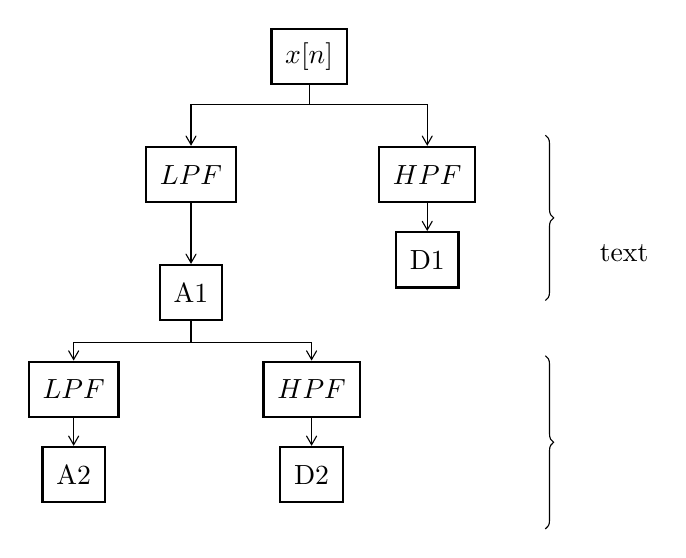
\begin{tikzpicture}[cell/.style={rectangle,draw, thick,align=center, minimum size=2em,inner sep=5pt}, input/.style={->}]

\node[cell] at (0,0) (xn) {$x[n]$};

\node[cell] at (-1.5,-1.5) (lpf1) {$LPF$};
\node[cell] at (1.5,-1.5) (hpf1){$HPF$};

\node[cell] at (-1.5,-3) (A1) {A1};
\node[cell, below = 1em of hpf1]  (D1) {D1};

\node[cell, below left = 2em of A1] (lpf2) {$LPF$};
\node[cell, below right = 2em of A1] (hpf2){$HPF$};

\node[cell, below = 1em of lpf2]  (A2) {A2};
\node[cell, below = 1em of hpf2]  (D2) {D2};

\draw[->, >=angle 60] (xn) -- ++(0,-1em) -- ++(0,-0.75em) -| (lpf1);
\draw[->, >=angle 60] (xn) -- ++(0,-1em) -- ++(0,-0.75em) -| (hpf1);

\draw[->, >=angle 60] (lpf1) -- (A1);
\draw[->, >=angle 60] (hpf1) -- (D1);

\draw[->, >=angle 60] (A1) -- ++(0,-1em) -- ++(0,-0.8em) -| (lpf2);
\draw[->, >=angle 60] (A1) -- ++(0,-1em) -- ++(0,-0.8em) -| (hpf2);

\draw[->, >=angle 60] (lpf2) -- (A2);
\draw[->, >=angle 60] (hpf2) -- (D2);

\node[] at (3,-0.9) (coord1) {};
\node[] at (3,-3.25) (coord2) {};

\draw [decorate,decoration={brace,amplitude=3pt}] (3,-1) --  (3,-3.1) ;
\node at (4,-2.5) {text};
\draw [decorate,decoration={brace,amplitude=3pt}] (3,-3.8) --  (3,-6) ;
\end{tikzpicture}



	
\end{document}